\documentclass[11pt]{article}

% Required package
\usepackage{tikz}
\usepackage{fancyvrb, mdframed, verbatimbox, xcolor}
\usepackage{arrayjob}
\usepackage{calc}
%\usepackage{smartdiagram}
\usepackage[margin=0.5in]{geometry}
\usetikzlibrary{shapes.geometric, positioning, arrows.meta, calc, fit}


\tikzset{
	method/.style = {
		minimum width=3cm,
		minimum height=0.5cm,
		draw,
		align=flush left,
		text width=2.7cm,
	},
	type/.style = {
		minimum width=3cm,
		draw,
		align=center,
		text width=2.7cm,
	}
}

\tikzset{frame/.style={line width=0.1mm, inner sep=0.9em, draw=#1}}

\begin{document}
	\begin{figure}[h!]
		\caption{OCPConform}
	\begin{mdframed}
		\centering
		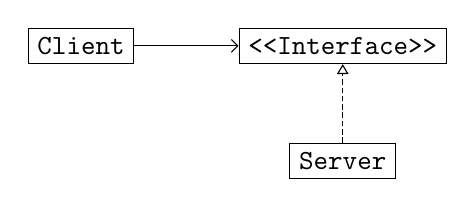
\begin{tikzpicture}

		\node[rectangle,draw] (client) at (0,0) {\Verb|Client|};

		\node[rectangle,draw] (interface) [right=2cm] {\Verb|<<Interface>>|};

		\node[rectangle,draw] (server) [below=1cm of interface,] {\Verb|Server|};

		\draw[-Straight Barb] (client.east) -- (interface.west);

		\draw[dash pattern=on 2pt off 1pt, -{Triangle[open]}] (server.north) -- (interface.south);

	\end{tikzpicture}
	\end{mdframed}
	\end{figure}

	\begin{figure}[h!]
		\caption{OCPViolate}
		\begin{mdframed}
			\centering
			
\begin{tikzpicture}

				\node[rectangle,draw] (client) at (0,0) {\Verb|Client|};

				\node[rectangle,draw] (server) [right=of client,] {\Verb|Server|};

				\draw[-Straight Barb] (client) -- (server);

			\end{tikzpicture}
		\end{mdframed}
	\end{figure}

	\begin{figure}[h!]
		\caption{Adapter}
	\begin{mdframed}
		\centering
		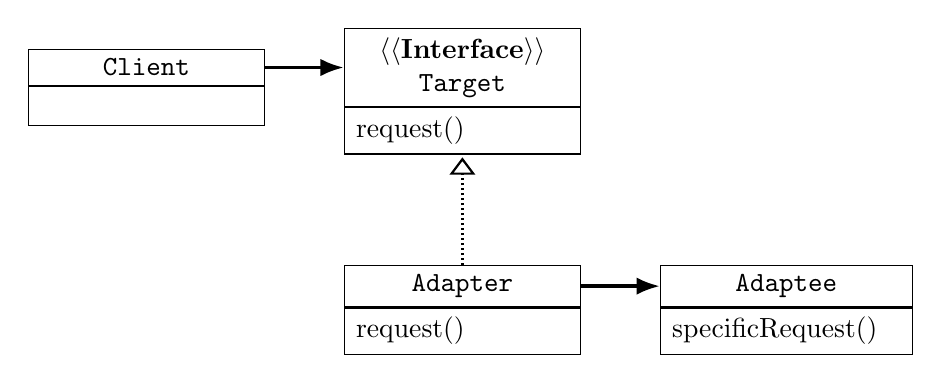
\begin{tikzpicture}
		\node[type] (target) {
			\textbf{$ \langle\langle $Interface$ \rangle\rangle $} \\
			\Verb|Target|};

		\node[method] (request) [below=0pt of target] {request()};

		\node[type] (client) [left=of target] {\Verb|Client|};
		\node[method] () [below=0pt of client] {};

		\draw[very thick, -Latex] (client.east) -- (target.west);

		\node[type] (adapter) [below=2cm of target] {\Verb|Adapter|};
		\node[method] () [below=0pt of adapter] {request()};

		\node[type, minimum width=3.2cm] (adaptee) [right=of adapter] {\Verb|Adaptee|};
		\node[method, minimum width=3.2cm, text width=2.9cm] () [below=0pt of adaptee] {specificRequest()};

		\draw[densely dotted,-{Triangle[open, width=2.5mm, scale=1.3]}, shorten >= 1pt, thick] (adapter.north) -- (request.south);
		\draw[very thick, -Latex] (adapter.east) -- (adaptee.west);
	\end{tikzpicture}
	\end{mdframed}
	\end{figure}

	\begin{figure}[h!]
		\caption{DIPConform}
	\begin{mdframed}
		\centering
		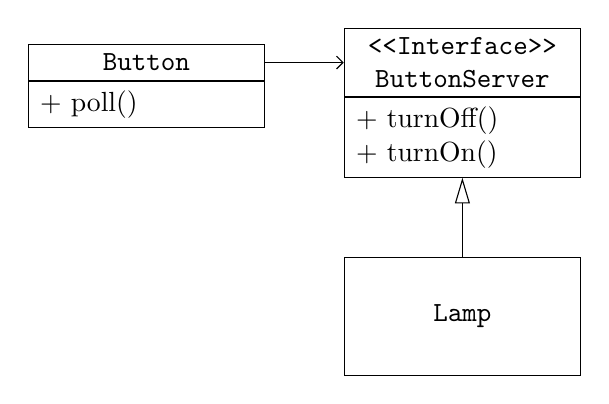
\begin{tikzpicture}
			\node[type] (buttonserver) {\Verb|<<Interface>>|\\
			\Verb|ButtonServer|};
			\node[method] (serverfn) [below=0pt of buttonserver] {+ turnOff()\\
			+ turnOn()};

			\node[type] (button) [left=of buttonserver] {\Verb|Button|};
			\node[method] () [below=0pt of button] {+ poll()};

			\node[type, minimum height=1.5cm] (lamp) [below=of serverfn] {\Verb|Lamp|};

			\draw[-Straight Barb] (button) -- (buttonserver);
			\draw[-{Triangle[open, length=2.5mm, scale=1.3]}] (lamp) -- (serverfn);
		\end{tikzpicture}
	\end{mdframed}
	\end{figure}

	\begin{figure}[h!]
		\caption{DIPViolate}
	\begin{mdframed}
		\centering
		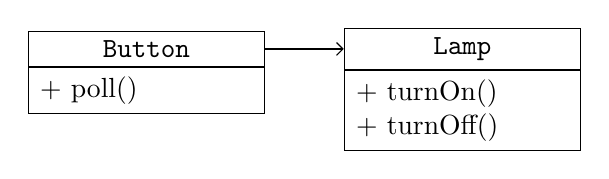
\begin{tikzpicture}
			\node[type] (lamp) {\Verb|Lamp|};
			\node[method] () [below=0pt of lamp] {+ turnOn()\\
			+ turnOff()};

			\node[type] (button) [left=of lamp] {\Verb|Button|};
			\node[method] () [below=0pt of button] {+ poll()};

			\draw[-Straight Barb] (button) -- (lamp);
		\end{tikzpicture}
	\end{mdframed}
	\end{figure}

	\begin{figure}[h!]
		\caption{DIPNaive}
	\begin{mdframed}
		\centering
		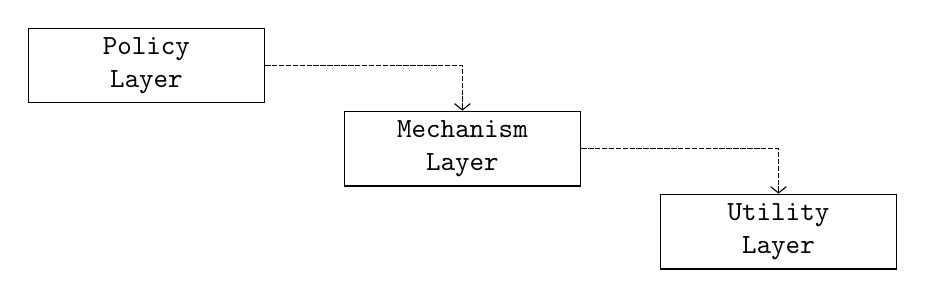
\begin{tikzpicture}
			\node[type] (mechanism) {\Verb|Mechanism| \\ \Verb|Layer|};
			\node[type] (policy) [left=of mechanism, yshift=30pt]{\Verb|Policy| \\ \Verb|Layer|};
			\node[type] (utility) [right=of mechanism, yshift=-30pt] {\Verb|Utility| \\ \Verb|Layer|};

			\draw[dash pattern=on 2pt off 0.5pt, -{Straight Barb[width=2mm]}] (policy.east) -| (mechanism.north);
			\draw[dash pattern=on 2pt off 0.5pt, -{Straight Barb[width=2mm]}] (mechanism.east) -| (utility.north);
		\end{tikzpicture}
	\end{mdframed}
	\end{figure}

	\begin{figure}[h!]
		\caption{DIPInverted}
		\begin{mdframed}
			\centering
			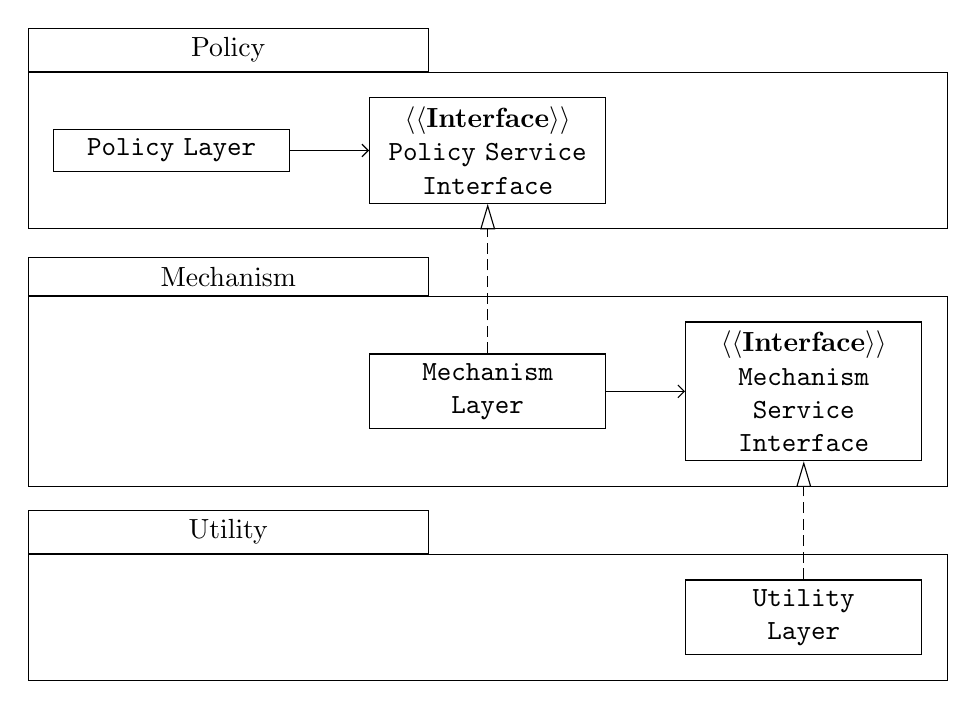
\begin{tikzpicture}
				\node[type] (mechanism) {\Verb|Mechanism| \\ \Verb|Layer|};
				\node[type] (mechinterface) [right=of mechanism] {\textbf{$ \langle\langle $Interface$ \rangle\rangle $} \\ \Verb|Mechanism| \\ \Verb|Service| \\ \Verb|Interface|};
				\node[minimum width=3cm] [left=of mechanism] (ghostmech) {};

				\draw[-Straight Barb] (mechanism) -- (mechinterface);

				\node[type] (policyinterface) [above=1.9cm of mechanism] {\textbf{$ \langle\langle $Interface$ \rangle\rangle $} \\ \Verb|Policy Service| \\ \Verb|Interface|};
				\node[type] (policy) [left=of policyinterface] {\Verb|Policy Layer|};
				\node[minimum width=3cm] [right=of policyinterface] (ghostpolicy) {};

				\draw[-Straight Barb] (policy) -- (policyinterface);
				\draw[dash pattern=on 4pt off 2pt, -{Triangle[open, length=2.5mm, scale=1.3]}] (mechanism) -- (policyinterface);

				\node[type] (utilityinterface) [below=1.5cm of mechinterface] {\Verb|Utility| \\ \Verb|Layer|};
				\node[minimum width=3cm] (ghostutil1) [left=of utilityinterface] {};
				\node[minimum width=3cm] (ghostutil2) [left=of ghostutil1] {};
				\draw[dash pattern=on 4pt off 2pt, -{Triangle[open, length=2.5mm, scale=1.3]}] (utilityinterface) -- (mechinterface);

				\node[frame=black, fit=(mechanism)(mechinterface)(ghostmech)] (mech) {};
				\node[frame=black, fit=(policy)(policyinterface)(ghostpolicy)] (poli) {};
				\node[frame=black, fit=(utilityinterface)(ghostutil1)(ghostutil2)] (util) {};

				\node[draw, rectangle, above right, minimum width=2in] at (poli.north west) {Policy};
				\node[draw, rectangle, above right, minimum width=2in] at (mech.north west) {Mechanism};
				\node[draw, rectangle, above right, minimum width=2in] at (util.north west) {Utility};
			\end{tikzpicture}
		\end{mdframed}
	\end{figure}

	\begin{figure}[h!]
		\caption{Compile flow}
		\begin{mdframed}
			\centering
			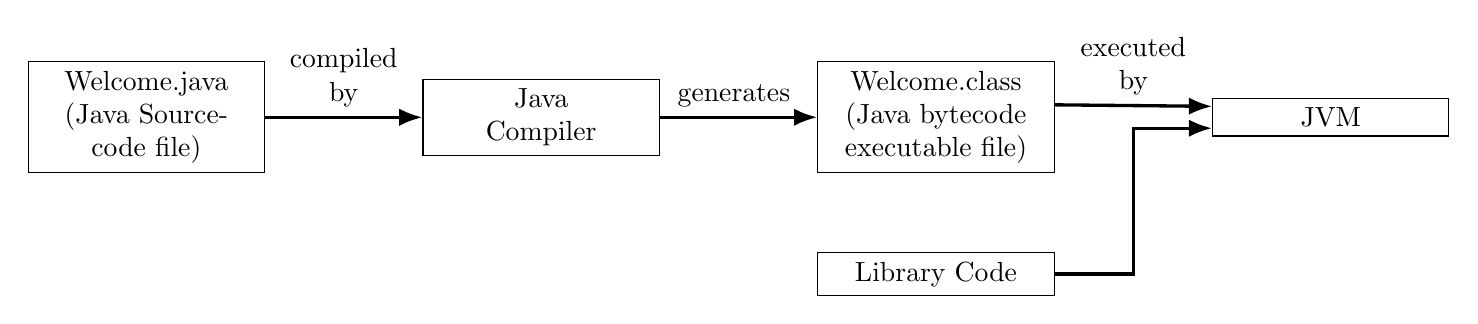
\begin{tikzpicture}
				\node[type] (welcome) {Welcome.java \\ (Java Source- \\ code file)};
				\node[type] (compiler) [right=2cm of welcome] {Java \\ Compiler};
				\node[type] (welcomeclass) [right=2cm of compiler] {Welcome.class \\ (Java bytecode \\ executable file)};
				\node[type] (jvm) [right=2cm of welcomeclass] {JVM};
				\node[type] (library) [below=of welcomeclass] {Library Code};

				\draw[very thick, -Latex] (welcome) -- (compiler)
					node[above, align=center, midway] {
						compiled\\
						by
					};
				\draw[very thick, -Latex] (compiler) -- (welcomeclass)
					node[above, align=center, midway] {
						generates
					};
				\draw[very thick, -Latex] ([yshift=4.5pt]welcomeclass.east) -- ([yshift=-3pt]jvm.north west)
					node[above, align=center, midway] {
						executed\\
						by
					};
				\draw[very thick, -Latex] (library.east) -- +(1,0) |-  ([yshift=3pt]jvm.south west);
			\end{tikzpicture}
		\end{mdframed}
	\end{figure}

	\begin{figure}[h!]
		\caption{ISPViolation}
		\begin{mdframed}
			\centering
			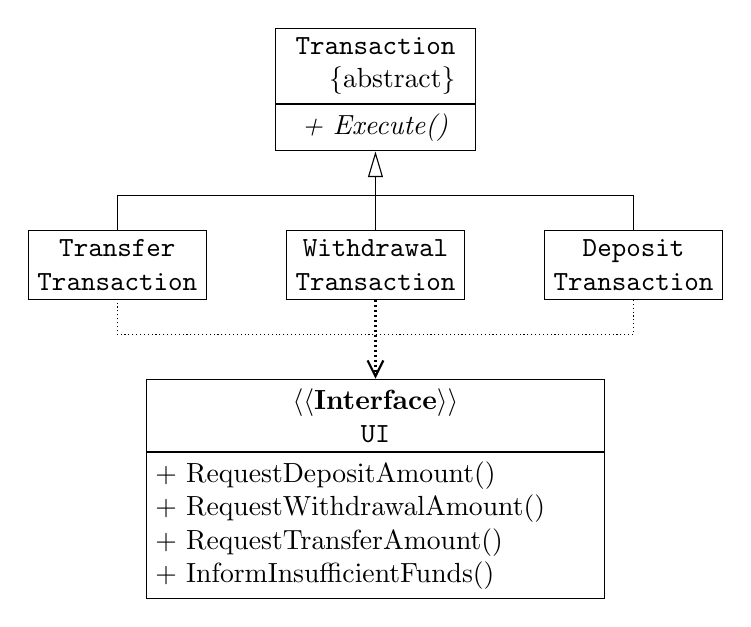
\begin{tikzpicture}
				\node[rectangle, align=center, draw] (withdrawal) {\Verb|Withdrawal| \\ \Verb|Transaction|};
				\node[rectangle, align=center, draw] (deposit) [right=of withdrawal]{\Verb|Deposit| \\ \Verb|Transaction|};
				\node[rectangle, align=center, draw] (transfer) [left=of withdrawal] {\Verb|Transfer| \\ \Verb|Transaction|};

				\node[rectangle, align=left, draw, minimum width=1in] (withdrawaltype) [above=of withdrawal] {\textit{+ Execute()}};
				\node[rectangle, align=right, draw, minimum width=1in] (transaction) [above=0pt of withdrawaltype] {\Verb|Transaction| \\ \{abstract\}};
				\coordinate (ghost) [above= 10pt of withdrawal] {};

				\draw (deposit.north) |- ([yshift=25pt]ghost) -| (transfer.north);
				\draw[-{Triangle[open, length=2.5mm, scale=1.3]}] (withdrawal) -- (withdrawaltype);

				\node[type, text width=2.2in] (ui) [below=of withdrawal] {\textbf{$ \langle\langle $Interface$ \rangle\rangle $} \\ \Verb|UI|};
				\node[method, text width=2.2in] () [below=0pt of ui] {+ RequestDepositAmount() \\ + RequestWithdrawalAmount() \\ + RequestTransferAmount() \\ + InformInsufficientFunds()};
				\coordinate (ghost2) [below= 10pt of withdrawal] {};

				\draw[densely dotted] (deposit.south) |- ([yshift=-25pt]ghost2) -| (transfer.south);
				\draw[densely dotted, -{Straight Barb[length=2mm, width=2mm]}, thick] (withdrawal) -- (ui);
			\end{tikzpicture}
		\end{mdframed}
	\end{figure}

	\begin{figure}[h!]
		\caption{ISPObey}
		\begin{mdframed}
			\centering
			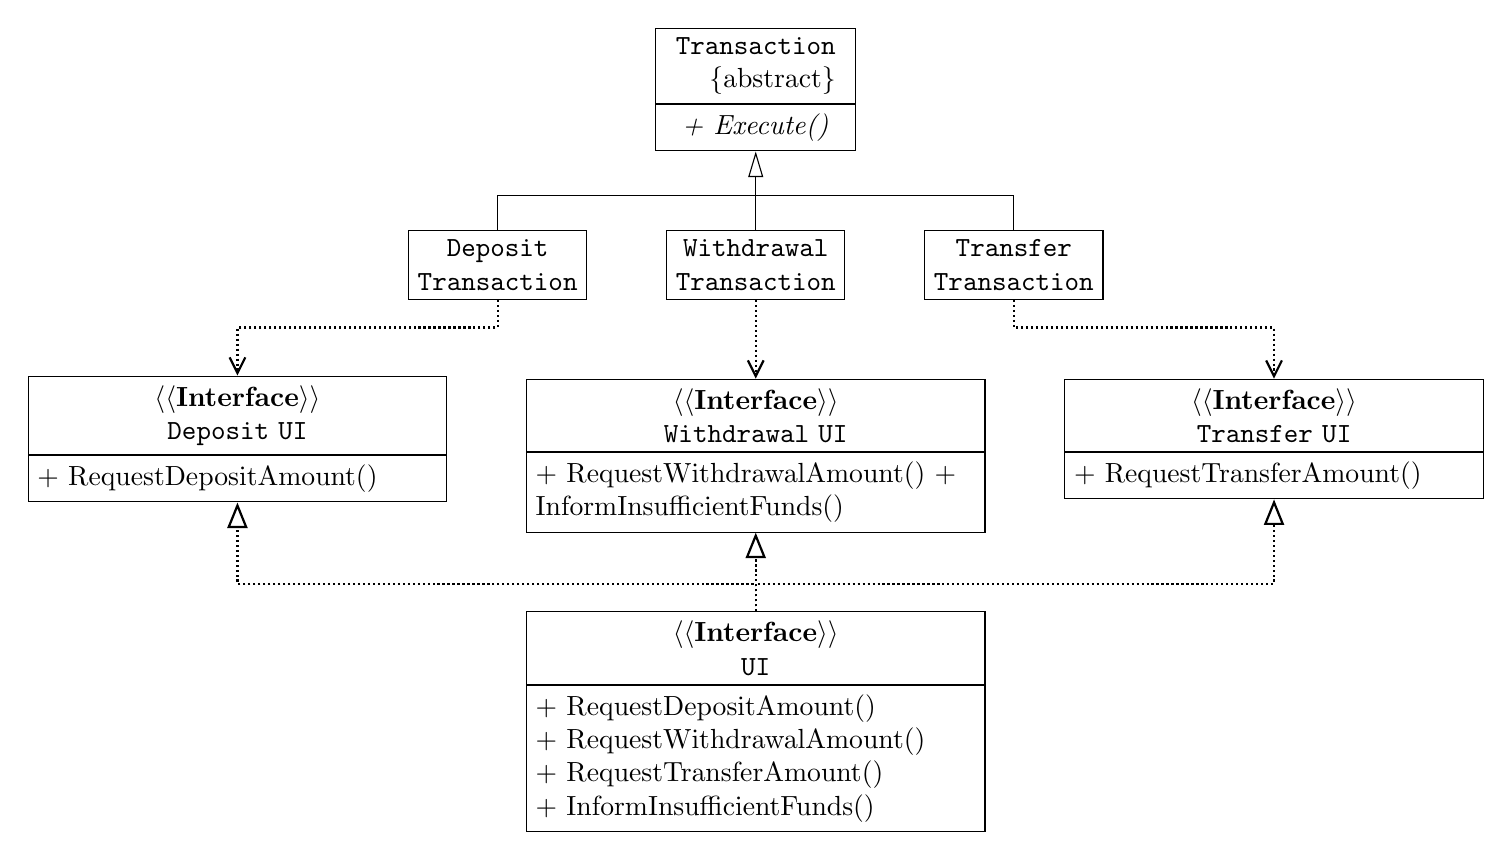
\begin{tikzpicture}
				\node[rectangle, align=center, draw] (withdrawal) {\Verb|Withdrawal| \\ \Verb|Transaction|};
				\node[rectangle, align=center, draw] (deposit) [left=of withdrawal]{\Verb|Deposit| \\ \Verb|Transaction|};
				\node[rectangle, align=center, draw] (transfer) [right=of withdrawal] {\Verb|Transfer| \\ \Verb|Transaction|};

				\node[rectangle, align=left, draw, minimum width=1in] (withdrawaltype) [above=of withdrawal] {\textit{+ Execute()}};
				\node[rectangle, align=right, draw, minimum width=1in] (transaction) [above=0pt of withdrawaltype] {\Verb|Transaction| \\ \{abstract\}};
				\coordinate (ghost) [above= 10pt of withdrawal] {};

				\draw (deposit.north) |- ([yshift=25pt]ghost) -| (transfer.north);
				\draw[-{Triangle[open, length=2.5mm, scale=1.3]}] (withdrawal) -- (withdrawaltype);

				\node[type, text width=2.2in] (wui) [below=of withdrawal] {\textbf{$ \langle\langle $Interface$ \rangle\rangle $} \\ \Verb|Withdrawal UI|};
				\node[method, text width=2.2in] (wtype) [below=0pt of wui] {+ RequestWithdrawalAmount() + InformInsufficientFunds()};

				\node[type, text width=2in] (dui) [left=of wui] {\textbf{$ \langle\langle $Interface$ \rangle\rangle $} \\ \Verb|Deposit UI|};
				\node[method, text width=2in] (dtype) [below=0pt of dui] {+ RequestDepositAmount()};

				\node[type, text width=2in] (tui) [right=of wui] {\textbf{$ \langle\langle $Interface$ \rangle\rangle $} \\ \Verb|Transfer UI|};
				\node[method, text width=2in] (ttype) [below=0pt of tui] {+ RequestTransferAmount()};

				\draw[densely dotted, -{Straight Barb[length=2mm, width=2mm]}, thick] (withdrawal) -- (wui);
				\draw[densely dotted, -{Straight Barb[length=2mm, width=2mm]}, thick] (deposit.south) -- ([yshift=-10pt]deposit.south) -| (dui);
				\draw[densely dotted, -{Straight Barb[length=2mm, width=2mm]}, thick] (transfer.south) -- ([yshift=-10pt]transfer.south) -| (tui);

				\node[type, text width=2.2in] (ui) [below=of wtype] {\textbf{$ \langle\langle $Interface$ \rangle\rangle $} \\ \Verb|UI|};
				\node[method, text width=2.2in] () [below=0pt of ui] {+ RequestDepositAmount() \\ + RequestWithdrawalAmount() \\ + RequestTransferAmount() \\ + InformInsufficientFunds()};

				\draw[densely dotted, -{Triangle[open, length=2.5mm, scale=1.3]}, thick] (ui) -- (wtype);
				\draw[densely dotted, -{Triangle[open, length=2.5mm, scale=1.3]}, thick] (ui) -- ([yshift=10pt]ui.north) -| (dtype);
				\draw[densely dotted, -{Triangle[open, length=2.5mm, scale=1.3]}, thick] (ui) -- ([yshift=10pt]ui.north) -| (ttype);
			\end{tikzpicture}
		\end{mdframed}
	\end{figure}

\begin{verbbox}[\small]
if (x < y)
{
  y = 0;
  x = x + 1;
}
else
{
  x = y;
}
\end{verbbox}
	\begin{figure}
		\caption{CFG}
		\begin{mdframed}
			\centering
			$\vcenter{\hbox{\theverbbox}}$ \quad
			$\vcenter{\hbox{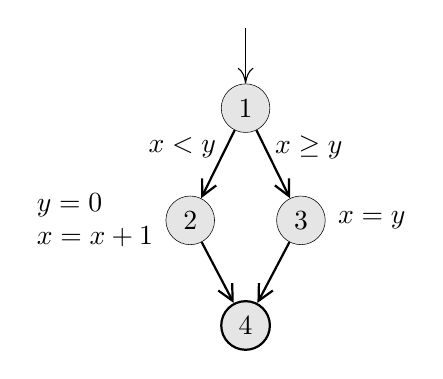
\begin{tikzpicture}[mycircle/.style={circle, fill=gray!20, draw, very thin}]
				\node[mycircle] (one) {1};
				\draw[-{To[length=2mm, width=2mm]}] ([yshift=20pt]one.north) -- (one.north);

				\node[mycircle] (two) [below=0.8cm of one, xshift=-20pt] {2};
				\node[mycircle] (three) [below=0.8cm of one, xshift=20pt] {3};
				\draw[-{Straight Barb[length=2mm, width=2mm]}, thick] (one) -- (two) node[left, near start] {$ x < y $};
				\draw[-{Straight Barb[length=2mm, width=2mm]}, thick] (one) -- (three) node[right, near start] {$ x \geq y $};
				\node [right=1pt of three] {$ x = y $};
				\node[align=left] [left=1pt of two] {$ y = 0 $ \\ $ x = x +1 $};

				\node[mycircle, thick] (four) [below=0.7cm of two, xshift=20pt] {4};
				\draw[-{Straight Barb[length=2mm, width=2mm]}, thick] (two) -- (four);
				\draw[-{Straight Barb[length=2mm, width=2mm]}, thick] (three) -- (four);
			\end{tikzpicture}}}$
		\end{mdframed}
	\end{figure}

	\begin{figure}[h!]
		\caption{MVP}
		\begin{mdframed}
			\centering
			\definecolor{MVPBlue}{HTML}{5b9ad5}
			\begin{tikzpicture}
				\node[type, rounded corners, fill=MVPBlue, text=white] (Presenter) {{\Large Presenter}};
				\node[type, rounded corners, fill=MVPBlue, text=white] (Model) [above=of Presenter] {{\Large Model}};
				\node[type, rounded corners, fill=MVPBlue, text=white] (View) [below=of Presenter] {{\Large View}};

				\draw[-Latex, thick] ([xshift=10pt]Presenter.north west) -- ([xshift=10pt]Model.south west) node[left, midway, align=left] {Update \\ Model};
				\draw[-Latex, thick] ([xshift=10pt]Presenter.south west) -- ([xshift=10pt]View.north west) node[left, midway, align=left] {Update \\ UI};

				\draw[-Latex, thick]  ([xshift=-10pt]View.north east) -- ([xshift=-10pt]Presenter.south east) node[right, midway, align=left] {User \\ Events};
				\draw[-Latex, thick]  ([xshift=-10pt]Model.south east) -- ([xshift=-10pt]Presenter.north east) node[right, midway, align=left] {Model-change \\ Events};
			\end{tikzpicture}
		\end{mdframed}
	\end{figure}

	\begin{figure}[h!]
		\caption{SDLCCircle}
		\begin{mdframed}
			\centering
			\definecolor{MVPBlue}{HTML}{5b9ad5}
			\begin{tikzpicture}
				\def \n {5}
				\def \radius {3.5cm}
				\def \margin {8} % margin in angles, depends on the radius
				\newarray\SDLC
				\readarray{SDLC}{Design&Analysis&Planning&Maintenance&Implementation}%
				\foreach \s in {1,...,\n}
				{
					\node[minimum width=3cm, rounded corners, fill=MVPBlue, text=white, minimum height=1cm] (s\s) at ({360/\n * (\s - 1) + 18}:\radius) {\SDLC(\s)};
				}
%				\draw[->] (s1.north) arc (90:0:3.5);
%				\draw[->] (s2.west) to[out=190, in=90] (s3);
				\draw[-Latex, thick] (s1.north) -- (s2.east);
				\draw[-Latex, thick] (s2.west) -- (s3.north);
				\draw[-Latex, thick] (s3.south) -- (s4.north);
				\draw[-Latex, thick] (s4.east) -- (s5.west);
				\draw[-Latex, thick] (s5.north) -- (s1.south);
			\end{tikzpicture}
%			\tikzset{
%				every shadow/.style={
%					fill=none,
%					shadow xshift=0pt,
%					shadow yshift=0pt}
%			}
%
%			\tikzset{module/.append style={top color=MVPBlue,bottom color=MVPBlue}}
%			\smartdiagramset{uniform color list=MVPBlue for 5 items,
%				arrow line width=2pt,
%				text width=1.3in,
%				text color=white,
%				font=\normalsize
%			}
%			\smartdiagram[circular diagram:clockwise]{Design,Analysis,Planning,Maintenance,Implementation}
		\end{mdframed}
	\end{figure}

	\begin{figure}
		\caption{LSPExample}
		\begin{mdframed}
			\centering
			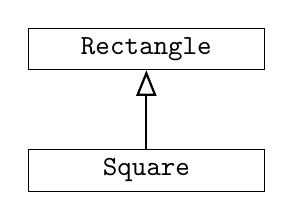
\begin{tikzpicture}
				\node[type] (Square) {\Verb|Square|};
				\node[type] (Rectangle) [above=of Square] {\Verb|Rectangle|};

				\draw[thick, -{Triangle[open, length=2.5mm, scale=1.3]}] (Square) -- (Rectangle);
			\end{tikzpicture}
		\end{mdframed}
	\end{figure}

	\begin{figure}[h!]
		\caption{Observer}
		\begin{mdframed}
			\centering
			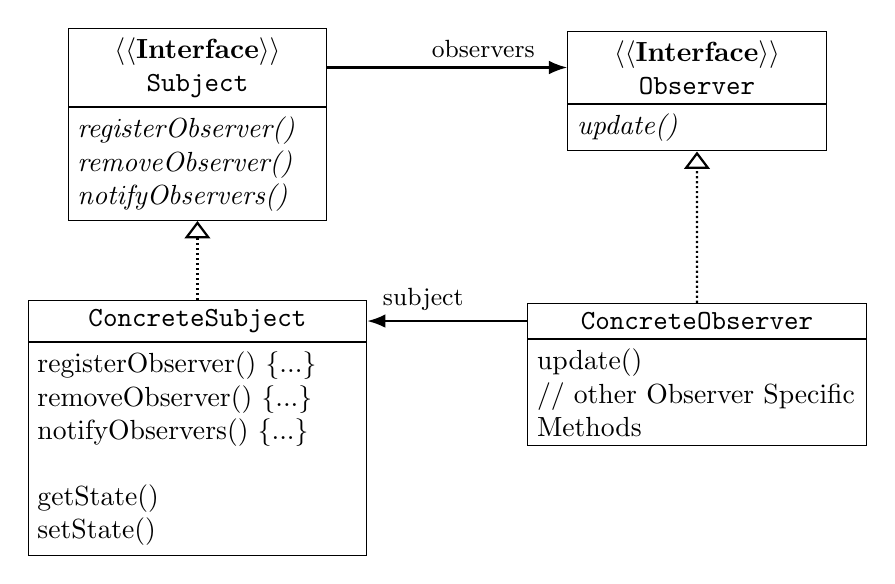
\begin{tikzpicture}
				\node[type, text width=1.2in] (subject) {\textbf{$ \langle\langle $Interface$ \rangle\rangle $} \\ \Verb|Subject|};
				\node[method, text width=1.2in, align=left] (stype) [below=0pt of subject] {\textit{registerObserver()} \\ \textit{removeObserver()} \\ \textit{notifyObservers()}};

				\node[type, text width=1.2in] (observer) [right=1.2in of subject] {\textbf{$ \langle\langle $Interface$ \rangle\rangle $} \\ \Verb|Observer|};
				\node[method, text width=1.2in, align=left] (otype) [below=0pt of observer] {\textit{update()}};

				\node[type, text width=1.6in] (consubject) [below=of stype]{\Verb|ConcreteSubject|};
				\node[method, text width=1.6in, align=left] (ctype) [below=0pt of consubject] {{registerObserver() \{...\}} \\ {removeObserver() \{...\}} \\ {notifyObservers() \{...\}} \\ \phantom{Empty space} \\ getState() \\ setState()};

				\node[type, text width=1.6in] (conobserver) [right=0.8in of consubject] {\Verb|ConcreteObserver|};
				\node[method, text width=1.6in] (cotype) [below=0pt of conobserver] {update() \\ // other Observer Specific \\ Methods};

				\draw[-Latex, thick] (subject) -- (observer) node[above, pos=0.65] () {{\small observers}};
				\draw[-Latex, thick] (conobserver) -- (consubject) node[above, pos=0.65] () {{\small subject}};
				\draw[densely dotted,-{Triangle[open, width=2.5mm, scale=1.3]}, thick] (consubject) -- (stype);
				\draw[densely dotted,-{Triangle[open, width=2.5mm, scale=1.3]}, thick] (conobserver) -- (otype);
			\end{tikzpicture}
		\end{mdframed}
	\end{figure}

	\begin{figure}[h!]
		\caption{SRPConform}
		\begin{mdframed}
			\centering
			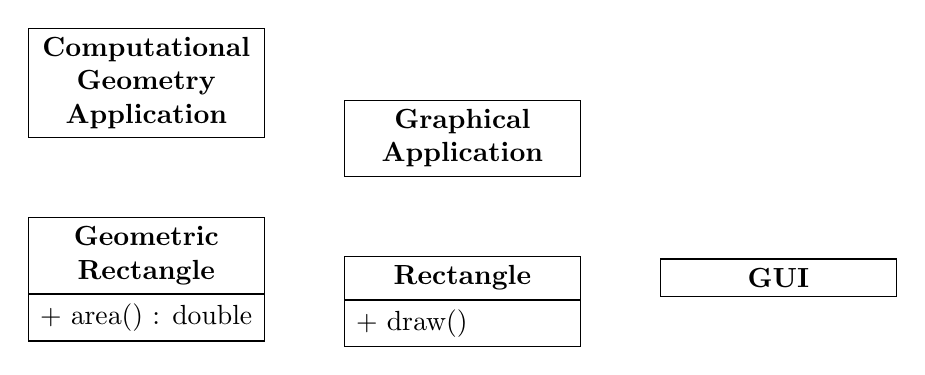
\begin{tikzpicture}
				\node[type, anchor=north west] (rectangle) {\textbf{Rectangle}};
				\node[method] (rtype) [below=0pt of rectangle] {+ draw()};

				\node[type] (gui) [right=of rectangle] {\textbf{GUI}};
				\node[type] (graphapp) [above=of rectangle] {\textbf{Graphical} \\ \textbf{Application}};

				\node[type,anchor=north west] (geom) [left=of rectangle.north west] {\textbf{Geometric} \\ \textbf{Rectangle}};
				\node[method] () [below=0pt of geom] {+ area() : double};

				\node[type] (geoapp) [above=of geom] {\textbf{Computational} \\ \textbf{Geometry} \\ \textbf{Application}};
			\end{tikzpicture}
		\end{mdframed}
	\end{figure}

	\begin{figure}[h!]
		\caption{LITests}
		\begin{mdframed}
			\centering
			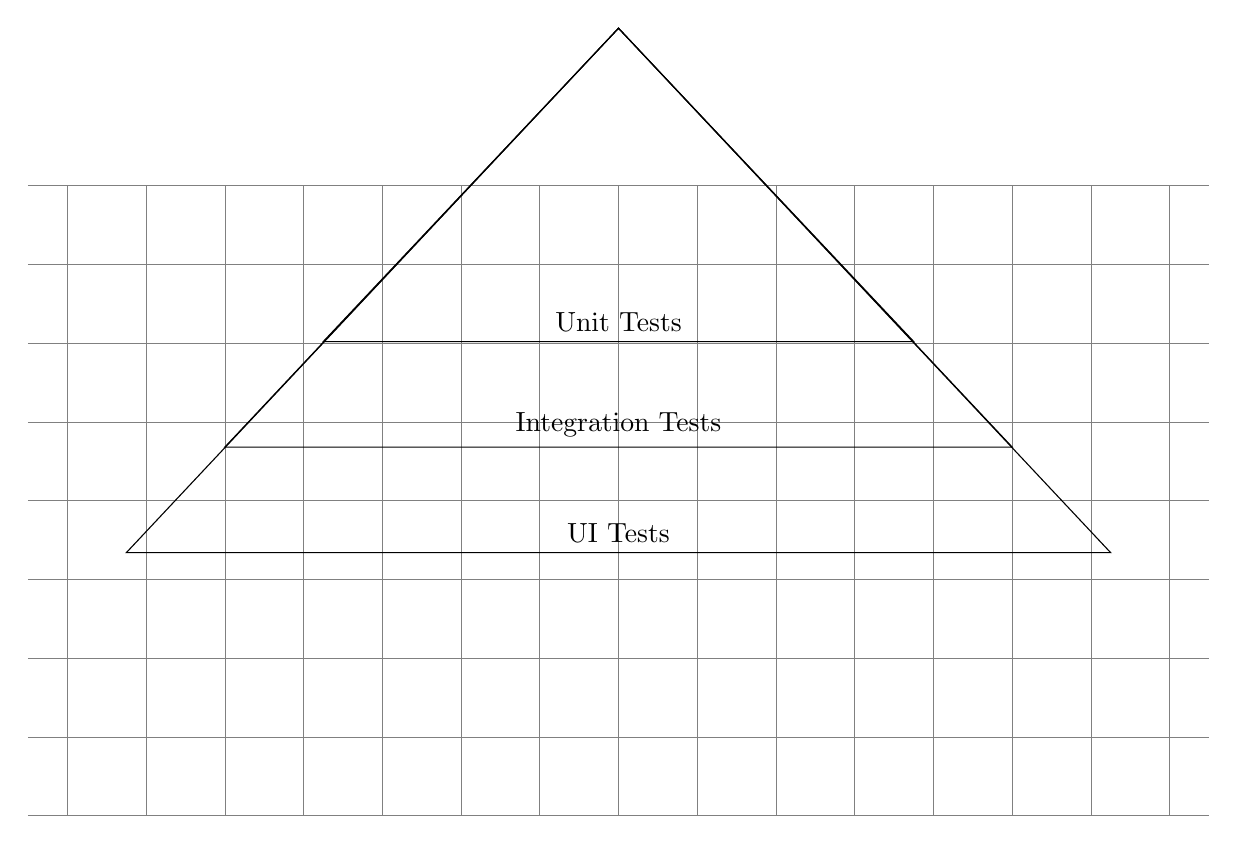
\begin{tikzpicture}[x=2.5cm,y=2cm]
				\draw[help lines] (-3,-2) grid (3, 2);
				\coordinate (A) at (-3,-1) {};
				\coordinate (B) at (3,-1) {};
				\coordinate (C) at (0,3) {};
				\foreach \A [count=\i] in {UI Tests, Integration Tests, Unit Tests}
				\draw[] (C)--([shift={(-.5*\i,0.67*\i)}]B)--node[above,align=center] {\A}([shift={(.5*\i,0.67*\i)}]A)--cycle;
			\end{tikzpicture}
		\end{mdframed}
	\end{figure}

	\begin{figure}[h!]
		\caption{Strategy}
		\begin{mdframed}
			\centering
			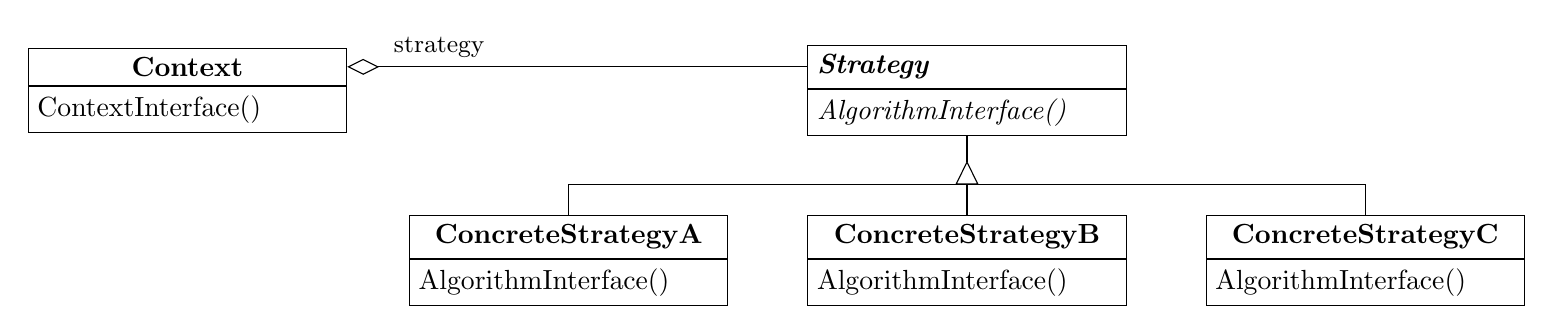
\begin{tikzpicture}
				\node[type, align=left, text width=1.5in] (strategy) {\textit{\textbf{Strategy}}};
				\node[method, text width=1.5in] (stratmeth) [below=0pt of strategy] {\textit{AlgorithmInterface()}};

				\node[type, text width=1.5in] (stratb) [below=of stratmeth] {\textbf{ConcreteStrategyB}};
				\node[method, text width=1.5in] () [below=0pt of stratb] {AlgorithmInterface()};

				\node[type, text width=1.5in] (stratc) [right=of stratb] {\textbf{ConcreteStrategyC}};
				\node[method, text width=1.5in] () [below=0pt of stratc] {AlgorithmInterface()};

				\node[type, text width=1.5in] (strata) [left=of stratb] {\textbf{ConcreteStrategyA}};
				\node[method, text width=1.5in] () [below=0pt of strata] {AlgorithmInterface()};

				\node[type, text width=1.5in] (context) [left=2.3in of strategy] {\textbf{Context}};
				\node[method, text width=1.5in] () [below=0pt of context] {ContextInterface()};

				\draw[-{Triangle[open, length=1.5mm, scale=2]}] (stratb.north) -- ([yshift=19.5pt]stratb.north);
				\draw (strata.north) |- ([yshift=11pt]stratb.north) -| (stratc.north);
				\draw ([yshift=19pt]stratb.north) -- (stratmeth);

				\draw[-{Diamond[open, scale=2]}] (strategy) -- (context) node[above, pos=0.8] () {{\small strategy}};
			\end{tikzpicture}
		\end{mdframed}
	\end{figure}
	\begin{figure}[h!]
		\caption{View}
		\begin{mdframed}
			\centering
			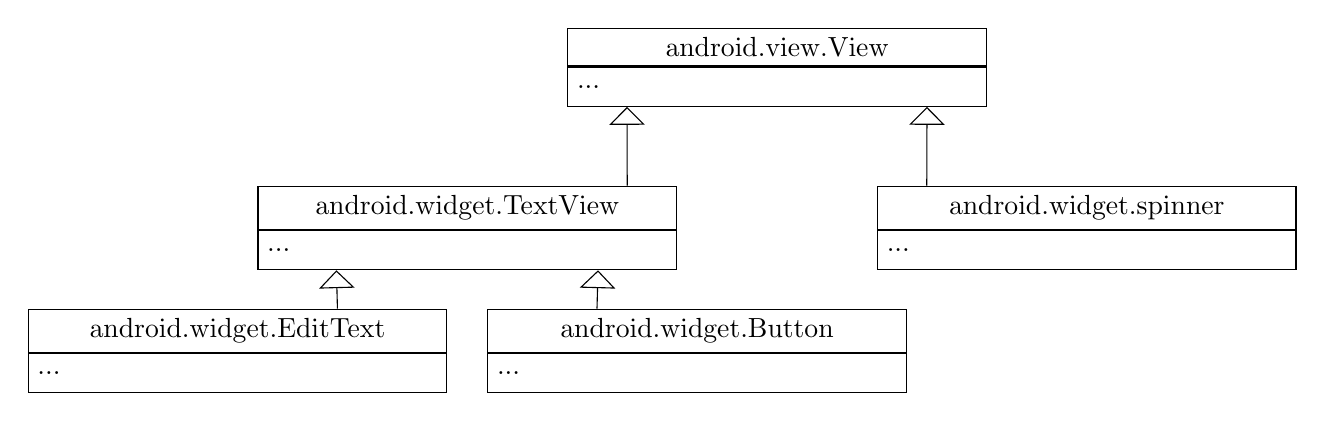
\begin{tikzpicture}
				\node[type, text width=2in] (head) {android.view.View};
				\node[method, text width=2in] (headtype) [below=0pt of head] {...};

				\node[type, text width=2in] (tv) [below=of headtype.south west, xshift=-0.5in] {android.widget.TextView};
				\node[method, text width=2in] (tvtype) [below=0pt of tv] {...};

				\node[type, text width=2in] (sp) [below=of headtype.south east, xshift=0.5in] {android.widget.spinner};
				\node[method, text width=2in] () [below=0pt of sp] {...};

				\node[type, text width=2in] (et) [below=of tv.south west, xshift=-0.1in] {android.widget.EditText};
				\node[method, text width=2in] () [below=0pt of et] {...};

				\node[type, text width=2in] (bt) [below=of tv.south east, xshift=0.1in] {android.widget.Button};
				\node[method, text width=2in] () [below=0pt of bt] {...};

				\draw[-{Triangle[open, width=2.5mm, scale=1.8]}] ([xshift=0.8in]tv.north) -- ([xshift=-0.75in]headtype.south);
				\draw[-{Triangle[open, width=2.5mm, scale=1.8]}] ([xshift=-0.8in]sp.north) -- ([xshift=0.75in]headtype.south);

				\draw[-{Triangle[open, width=2.5mm, scale=1.8]}] ([xshift=0.5in]et.north) -- ([xshift=-0.654in]tvtype.south);
				\draw[-{Triangle[open, width=2.5mm, scale=1.8]}] ([xshift=-0.5in]bt.north) -- ([xshift=0.654in]tvtype.south);
			\end{tikzpicture}
		\end{mdframed}
	\end{figure}

	\begin{figure}[h!]
		\caption{ViewGroup}
		\begin{mdframed}
			\centering
			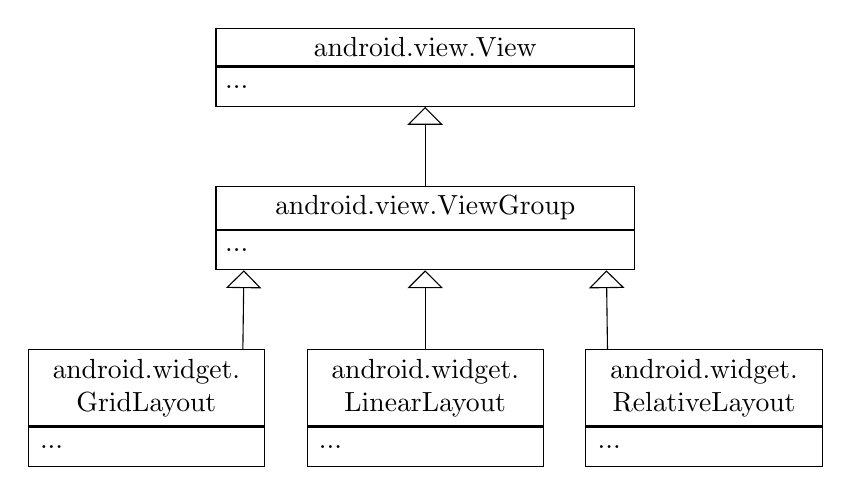
\begin{tikzpicture}
				\node[type, text width=2in] (vg) {android.view.ViewGroup};
				\node[method, text width=2in] (vgtype) [below=0pt of vg] {...};

				\node[method, text width=2in] (vtype) [above=of vg] {...};
				\node[type, text width=2in] (v) [above=0pt of vtype] {android.view.View};

				\node[type] (ll) [below=of vgtype] {android.widget. \\ LinearLayout};
				\node[method] () [below=0pt of ll] {...};

				\node[type] (gl) [left=15pt of ll] {android.widget. \\ GridLayout};
				\node[method] () [below=0pt of gl] {...};

				\node[type] (rl) [right=15pt of ll] {android.widget. \\ RelativeLayout};
				\node[method] () [below=0pt of rl] {...};

				\draw[-{Triangle[open, width=2.5mm, scale=1.8]}] (vg) -- (vtype);
				\draw[-{Triangle[open, width=2.5mm, scale=1.8]}] (ll) -- (vgtype);

				\draw[-{Triangle[open, width=2.5mm, scale=1.8]}] ([xshift=-8pt]gl.north east) -- ([xshift=10.3pt]vgtype.south west);
				\draw[-{Triangle[open, width=2.5mm, scale=1.8]}] ([xshift=8pt]rl.north west) -- ([xshift=-10.3pt]vgtype.south east);
			\end{tikzpicture}
		\end{mdframed}
	\end{figure}
\end{document}